\documentclass[aspectratio=169, lualatex, handout]{beamer}
\makeatletter\def\input@path{{theme/}}\makeatother\usetheme{cipher}

\title{Applied Cryptography - 2.3: Secure Messaging}
\author{Nadim Kobeissi}
\subject{An introduction to secure messaging protocols, covering the evolution from PGP through OTR to modern Signal, with focus on cryptographic properties, usability challenges, and implementation details.}
\keywords{secure messaging, cryptography, PGP, OTR, Signal, forward secrecy, deniability, authenticated key exchange, SIGMA, HKDF, usable security}
\institute{American University of Beirut}
\instituteimage{images/aub_white.png}
\date{\today}
\coversubtitle{CMPS 297AD/396AI\\Fall 2025}
\coverpartname{Part 2: Real-World Cryptography}
\covertopicname{2.3: Secure Messaging}
\coverwebsite{https://appliedcryptography.page}

\begin{document}
\begin{frame}[plain]
	\titlepage
\end{frame}

\section{The Dark Ages}

\begin{frame}{The Dark Ages}
	\begin{itemize}
		\item \textbf{Pretty Good Privacy} (PGP) - Created by Phil Zimmermann in 1991
		\item First widely available strong encryption for everyday people
		\item Uses public key cryptography for email encryption and digital signatures
		\item Revolutionary: Previously, strong crypto was government/military only
		\item Core idea: Each user has a key pair (public key + private key)
	\end{itemize}
\end{frame}

\begin{frame}{How PGP works}
	\begin{columns}
		\begin{column}{0.5\textwidth}
			\textbf{Encryption}
			\begin{enumerate}
				\item Alice writes email to Bob
				\item Gets Bob's public key
				\item PGP encrypts message with Bob's public key
				\item Only Bob's private key can decrypt
			\end{enumerate}
		\end{column}
		\begin{column}{0.5\textwidth}
			\textbf{Digital Signatures}
			\begin{enumerate}
				\item Alice signs with her private key
				\item Anyone with Alice's public key can verify
				\item Proves message came from Alice
				\item Detects tampering
			\end{enumerate}
		\end{column}
	\end{columns}
	\begin{alertblock}{Hybrid Encryption}
		Actually uses symmetric crypto for message, asymmetric for key exchange
	\end{alertblock}
\end{frame}

\begin{frame}{PGP in email clients}
	\begin{itemize}
		\item \textbf{Early days}: Command-line tools (1991-1995)
		      \begin{itemize}
			      \item Manual encryption/decryption
			      \item Copy and paste ciphertext into email
		      \end{itemize}
		\item \textbf{Integration era}: Plugins and extensions (1995-2010s)
		      \begin{itemize}
			      \item Enigmail for Thunderbird
			      \item GPGTools for Apple Mail
			      \item Outlook plugins
		      \end{itemize}
		\item \textbf{User experience}: Still complex!
		      \begin{itemize}
			      \item Key management burden on users
			      \item Accidental plaintext replies common
			      \item Attachments often forgotten
		      \end{itemize}
	\end{itemize}
\end{frame}

\begin{frame}{Look at this mess}
	\bigimagewithcaption{pgp_keyserver.png}{A PGP ``key server''}
\end{frame}

\begin{frame}{Look at this mess}
	\bigimagewithcaption{pgp_pubkey.png}{Allegedly my public key. Is it even? I don't know!}
\end{frame}

\begin{frame}{The Key Distribution Problem}
	\begin{columns}
		\begin{column}{0.6\textwidth}
			\textbf{How do you get someone's public key?}
			\begin{itemize}
				\item \textbf{Key servers}: MIT, SKS keyservers
				      \begin{itemize}
					      \item Upload your public key
					      \item Search by email/name
					      \item Anyone can upload anything!
				      \end{itemize}
				\item \textbf{Key fingerprints}: 40-hex-digit identifiers
				      \begin{itemize}
					      \item Verify out-of-band (phone, in person)
					      \item Business cards with fingerprints
				      \end{itemize}
				\item \textbf{Web of Trust}: Keys signed by other users
				      \begin{itemize}
					      \item ``I trust Alice, Alice trusts Bob''
					      \item Key signing parties!
					            \begin{itemize}
						            \item Such was our decadence, our confusion
					            \end{itemize}
				      \end{itemize}
			\end{itemize}
		\end{column}
		\begin{column}{0.4\textwidth}
			\begin{exampleblock}{Example Fingerprint}
				\ttfamily\scriptsize
				D745 2D8B 9E3F 4F3D\\
				7A82 F9B5 1C4A 6E9D\\
				8B3F 2E4C 9A7D 5F8E
			\end{exampleblock}
		\end{column}
	\end{columns}
\end{frame}

\begin{frame}{PGP: fundamental challenges}
	\begin{columns}[c]
		\begin{column}{1\textwidth}
			\begin{itemize}
				\item \textbf{Usability nightmare}
				      \begin{itemize}
					      \item ``Why Johnny Can't Encrypt'' (1999) - landmark usability study\footnote{\url{https://appliedcryptography.page/paper/\#johnny-cant}}
					      \item Key management too complex for average users
					      \item Easy to make catastrophic mistakes
				      \end{itemize}
				\item \textbf{No forward secrecy}
				      \begin{itemize}
					      \item Compromise private key = decrypt all past messages
					      \item Keys often used for years or decades
				      \end{itemize}
				\item \textbf{Metadata exposed}
				      \begin{itemize}
					      \item Subject lines, recipients visible
					      \item Timing and frequency observable
				      \end{itemize}
				\item \textbf{Web of Trust failed in practice}
				      \begin{itemize}
					      \item Most users never participated
				      \end{itemize}
			\end{itemize}
		\end{column}
	\end{columns}
\end{frame}

\begin{frame}{Why Johnny Can't Encrypt (1999)}
	\begin{columns}[T]
		\begin{column}{0.5\textwidth}
			\textbf{The Study}
			\begin{itemize}
				\item Whitten \& Tygar tested PGP 5.0
				\item 12 educated email users
				\item 90 minutes to encrypt/sign email
				\item Had manual + GUI interface
			\end{itemize}
			\textbf{Results: Catastrophic Failure}
			\begin{itemize}
				\item Only 1/3 succeeded
				\item 1/4 sent secrets in plaintext!
				\item Didn't understand public keys
				\item Used own key to encrypt to others
			\end{itemize}
		\end{column}
		\begin{column}{0.5\textwidth}
			\textbf{Core Conclusions}
			\begin{itemize}
				\item \textbf{Security $\neq$ normal software}
				      \begin{itemize}
					      \item Secondary goal for users
					      \item Mistakes are irreversible
					      \item Abstract concepts
				      \end{itemize}
				\item \textbf{Good GUI isn't enough}
				      \begin{itemize}
					      \item Need security-specific design
					      \item Must communicate mental model
				      \end{itemize}
				\item \textbf{``Usable security'' requires:}
				      \begin{itemize}
					      \item Users aware of security tasks
					      \item Can figure out how to do them
					      \item Don't make dangerous errors
					      \item Will continue using it
				      \end{itemize}
			\end{itemize}
		\end{column}
	\end{columns}
\end{frame}

\begin{frame}{Why Johnny Still, Still Can't Encrypt (2015)}
	\begin{columns}[T]
		\begin{column}{0.5\textwidth}
			\textbf{The Study - 16 Years Later}
			\begin{itemize}
				\item Ruoti et al. tested Mailvelope
				\item Modern PGP browser extension
				\item Integrates with webmail (Gmail)
				\item 20 participants (10 pairs)
				\item Exchange encrypted email
			\end{itemize}
			\textbf{Results: Still Catastrophic}
			\begin{itemize}
				\item \textbf{Only 1/10 pairs succeeded!}
				\item That pair took full 45 minutes
				\item Success only because one knew PKI
			\end{itemize}
		\end{column}
		\begin{column}{0.5\textwidth}
			\textbf{Common Failures}
			\begin{itemize}
				\item Encrypted with own public key (7/10)
				\item Generated keys with friend's info
				\item Recipients confused by PGP block
				\item One sent private key + password!
			\end{itemize}
			\textbf{Pain Points}
			\begin{itemize}
				\item No integrated tutorials
				\item PKI concepts still mystifying
				\item ``After 5 minutes, I would have just given up and called''
			\end{itemize}
		\end{column}
	\end{columns}
\end{frame}

\section{Off-the-Record Messaging: A Quick Summary}

\begin{frame}{Enter OTR: Off-the-Record Messaging}
	\begin{itemize}
		\item \textbf{Created in 2004} by Nikita Borisov, Ian Goldberg, and Eric Brewer
		\item Designed specifically for instant messaging, not email
		\item Key insight: Chat is synchronous, both parties online!
		\item \textbf{Revolutionary features}:
		      \begin{itemize}
			      \item Perfect forward secrecy
			      \item Deniable authentication
			      \item Automatic key exchange
		      \end{itemize}
	\end{itemize}
\end{frame}

\begin{frame}{OTR's take on key exchange}
	\begin{columns}
		\begin{column}{0.5\textwidth}
			\textbf{PGP's Problem}
			\begin{itemize}
				\item Need recipient's key \textit{before} messaging
				\item Complex key distribution infrastructure
				\item Users must understand PKI
				\item One key for all messages
			\end{itemize}
		\end{column}
		\begin{column}{0.5\textwidth}
			\textbf{OTR's Solution}
			\begin{itemize}
				\item Diffie-Hellman key agreement
				\item Keys negotiated per conversation
				\item Automatic and transparent
				\item New keys frequently (ratcheting)
			\end{itemize}
		\end{column}
	\end{columns}
\end{frame}

\begin{frame}{OTR: new security properties}
	\begin{itemize}
		\item \textbf{Forward Secrecy}
		      \begin{itemize}
			      \item Each message uses ephemeral keys
			      \item Compromise today doesn't reveal yesterday's messages
			      \item Keys deleted after use
		      \end{itemize}
		\item \textbf{Deniable Authentication}
		      \begin{itemize}
			      \item Messages authenticated to recipient
			      \item But no cryptographic proof for third parties
			      \item Like a real conversation - no permanent record
		      \end{itemize}
		\item \textbf{Socialist Millionaire Protocol}
		      \begin{itemize}
			      \item Verify identity without trusted third party
			      \item Share a secret question/answer
			      \item Zero-knowledge proof of shared knowledge
		      \end{itemize}
	\end{itemize}
\end{frame}

\begin{frame}{OTR integration success}
	\begin{columns}
		\begin{column}{0.6\textwidth}
			\textbf{Wide Platform Adoption}
			\begin{itemize}
				\item \textbf{Pidgin}: Multi-protocol IM client
				\item \textbf{Adium}: Mac OS X messaging
				\item \textbf{Kopete}: KDE instant messenger
				\item \textbf{Jitsi}: Voice/video/chat
			\end{itemize}
			\textbf{Protocol Support}
			\begin{itemize}
				\item XMPP/Jabber
				\item IRC (via proxy)
				\item AIM, ICQ, Yahoo Messenger
				\item Google Talk
			\end{itemize}
		\end{column}
		\begin{column}{0.4\textwidth}
			\textbf{Why It Worked}
			\begin{itemize}
				\item Plugin architecture
				\item No server changes needed
				\item Transparent to users
				\item ``Just works'' experience
				\item Graceful degradation
			\end{itemize}
		\end{column}
	\end{columns}
\end{frame}

\begin{frame}{OTR user experience}
	\begin{itemize}
		\item \textbf{Minimal user intervention}
		      \begin{itemize}
			      \item Click ``Start private conversation''
			      \item OTR negotiates automatically
			      \item Visual indicators show encryption status
		      \end{itemize}
		\item \textbf{Optional authentication}
		      \begin{itemize}
			      \item Can verify fingerprints if desired
			      \item Or use shared secret authentication
			      \item But works without it!
		      \end{itemize}
		\item \textbf{Clear security indicators}
		      \begin{itemize}
			      \item ``Private'' vs ``Not Private''
			      \item ``Verified'' vs ``Unverified''
			      \item Simple padlock icons
		      \end{itemize}
	\end{itemize}
\end{frame}

\begin{frame}{Pidgin: an IM client with OTR support}
	\bigimagewithcaption{pidgin_chat.jpg}{Pidgin supported MSN Messenger, Yahoo Messenger, IRC, etc.}
\end{frame}

\begin{frame}{Pidgin: an IM client with OTR support}
	\bigimagewithcaption{pidgin_otr.jpg}{Pidgin was a popular way to use OTR.}
\end{frame}

\begin{frame}{OTR's legacy}
	\begin{itemize}
		\item \textbf{Proved feasibility of usable crypto}
		      \begin{itemize}
			      \item Automatic key management works
			      \item Users don't need to understand crypto
			      \item Security can be transparent
		      \end{itemize}
		\item \textbf{Established core principles}
		      \begin{itemize}
			      \item Forward secrecy is essential
			      \item Ephemeral keys > long-term keys
			      \item Authentication without non-repudiation
		      \end{itemize}
		\item \textbf{Influenced modern messaging}
		      \begin{itemize}
			      \item Signal Protocol builds on OTR ideas
			      \item WhatsApp, Signal, Wire all use similar concepts
		      \end{itemize}
	\end{itemize}
\end{frame}

\section{Diving Into Secure Messaging Cryptography through OTR}

\begin{frame}{About this section}
	\begin{itemize}
		\item We're going to use OTR in order to start to understand how secure messaging protocols are designed.
		\item A core concept we're going to expand on in some detail: \textbf{authenticated key exchange}, especially how it applies to secure messaging protocols.
	\end{itemize}
\end{frame}

\begin{frame}{OTR: new security properties}{Reminder}
	\begin{itemize}
		\item \textbf{Forward Secrecy}
		      \begin{itemize}
			      \item Each message uses ephemeral keys
			      \item Compromise today doesn't reveal yesterday's messages
			      \item Keys deleted after use
		      \end{itemize}
		\item \textbf{Deniable Authentication}
		      \begin{itemize}
			      \item Messages authenticated to recipient
			      \item But no cryptographic proof for third parties
			      \item Like a real conversation - no permanent record
		      \end{itemize}
		\item \textbf{Socialist Millionaire Protocol}
		      \begin{itemize}
			      \item Verify identity without trusted third party
			      \item Share a secret question/answer
			      \item Zero-knowledge proof of shared knowledge
		      \end{itemize}
	\end{itemize}
\end{frame}

\begin{frame}{Regarding forward secrecy}
	\begin{itemize}
		\item \textbf{What is forward secrecy?}
		      \begin{itemize}
			      \item Past communications remain secure even if long-term keys are compromised
			      \item If attacker steals your keys today, they can't decrypt yesterday's messages
			      \item Critical property for long-lived messaging systems
		      \end{itemize}
		\item \textbf{How OTR achieves forward secrecy:}
		      \begin{enumerate}
			      \item Uses \textit{ephemeral} Diffie-Hellman key pairs
			      \item Keys relevant only for a small number of messages in the current conversation
			      \item Deleted immediately after use
			      \item New keys generated frequently (``ratcheting'')
		      \end{enumerate}
	\end{itemize}
\end{frame}

\begin{frame}{Regarding forward secrecy}
	\begin{itemize}
		\item Forward secrecy means that the protocol must:
		      \begin{enumerate}
			      \item Introduce a notion of \textit{ephemeral} public key pairs.
			      \item Use long-term key pairs (``identity keys'') \textit{only} in the AKE, and \textit{only} for authentication and identity binding, not in the ratcheting steps.
		      \end{enumerate}
	\end{itemize}
\end{frame}

\begin{frame}{Forward secrecy: key types}
	\begin{columns}
		\begin{column}{0.5\textwidth}
			\textbf{Long-term Identity Keys}
			\begin{itemize}
				\item Persist across sessions
				\item Identify users to each other
				\item Used only for authentication
				\item Never directly encrypt messages
				\item Compromise affects identity, not past messages
			\end{itemize}
		\end{column}
		\begin{column}{0.5\textwidth}
			\textbf{Ephemeral Keys}
			\begin{itemize}
				\item Generated per conversation
				\item Used for actual encryption
				\item Derived via Diffie-Hellman
				\item Deleted after use
				\item Cannot be recovered later
			\end{itemize}
		\end{column}
	\end{columns}
	\begin{alertblock}{Key Principle}
		Identity keys authenticate the key exchange, but ephemeral keys encrypt the messages
	\end{alertblock}
\end{frame}

\begin{frame}{Forward secrecy in practice}
	\begin{itemize}
		\item \textbf{The OTR approach:}
		      \begin{enumerate}
			      \item Alice and Bob perform authenticated DH exchange
			      \item Long-term keys sign the ephemeral public values
			      \item Shared secret derived from ephemeral keys only
			      \item Message keys derived from shared secret
			      \item All ephemeral material deleted after use
		      \end{enumerate}
		\item \textbf{Contrast with PGP:}
		      \begin{itemize}
			      \item PGP uses same key pair for years
			      \item One key compromise = all messages exposed
			      \item No automatic key rotation
		      \end{itemize}
	\end{itemize}
\end{frame}

\begin{frame}{SIGMA: SIGn-and-Mac Authenticated Key Exchange}
	\begin{columns}
		\begin{column}{0.4\textwidth}
			\begin{itemize}
				\item \textbf{AKE}
				      \begin{itemize}
					      \item Both parties verify each other's identity
					      \item Establish shared secret securely
				      \end{itemize}
				\item \textbf{Signatures for Authentication}
				      \begin{itemize}
					      \item Each party signs the DH ephemeral public keys
					      \item Prevents man-in-the-middle attacks
				      \end{itemize}
				\item $K_m \twoheadleftarrow \func{hash}{g^{xy}}$
			\end{itemize}
		\end{column}
		\begin{column}{0.6\textwidth}
			\begin{center}
				\begin{tikzpicture}[>=Stealth]
					\node (A) at (0,0) {$A$};
					\node (B) at (8,0) {$B$};
					\draw[->] (0.5,0) -- (7.5,0) node[midway,above] {$g^x$};
					\draw[<-] (0.5,-1) -- (7.5,-1) node[midway,above] {$g^y, g^B, \func{sign}{B, (g^x, g^y)}, \func{hmac}{K_m, g^B}$};
					\draw[->] (0.5,-2) -- (7.5,-2) node[midway,above] {$g^A, \func{sign}{A, (g^y, g^x)}, \func{hmac}{K_m, g^A}$};
				\end{tikzpicture}
			\end{center}
		\end{column}
	\end{columns}
\end{frame}

\begin{frame}{Why not this?}
	\begin{center}
		\begin{tikzpicture}[>=Stealth]
			\node (A) at (0,0) {$A$};
			\node (B) at (8,0) {$B$};
			\draw[->] (0.5,0) -- (7.5,0) node[midway,above] {$g^x$};
			\draw[<-] (0.5,-1) -- (7.5,-1) node[midway,above] {$g^y, g^B, \func{sign}{B, (g^x, g^y)}$};
			\draw[->] (0.5,-2) -- (7.5,-2) node[midway,above] {$g^A, \func{sign}{A, (g^y, g^x)}$};
		\end{tikzpicture}
	\end{center}
\end{frame}

\begin{frame}{Because\ldots}{Note that Bob records the exchange of the \textit{same} key with Eve that Alice exchanged with Bob!}
	\begin{center}
		\begin{tikzpicture}[>=Stealth]
			\node (A) at (0,0) {$A$};
			\node (B) at (8,0) {$B$};
			\draw[->] (0.5,0) -- (7.5,0) node[midway,above] {$g^x$};
			\draw[<-] (0.5,-1) -- (7.5,-1) node[midway,above] {$g^y, g^B, \func{sign}{B, (g^x, g^y)}$};
			\draw[->, red] (0.5,-2) -- (7.5,-2) node[midway,above] (crossed) {\textcolor{red}{$g^A, \func{sign}{A, (g^y, g^x)}$}};
			\draw[red, thick] (crossed.south west) -- (crossed.north east);
			\draw[->] (0.5,-2.7) -- (7.5,-2.7) node[midway,above] {$g^E, \func{sign}{E, (g^y, g^x)}$};
		\end{tikzpicture}
	\end{center}
\end{frame}

\begin{frame}{But why HMAC though?}{Why not just add the identity key to the signature?}
	\begin{center}
		\begin{tikzpicture}[>=Stealth]
			\node (A) at (0,0) {$A$};
			\node (B) at (8,0) {$B$};
			\draw[->] (0.5,0) -- (7.5,0) node[midway,above] {$g^A, g^x$};
			\draw[<-] (0.5,-1) -- (7.5,-1) node[midway,above] {$g^B, g^y, \func{sign}{B, (g^x, g^y, g^A)}$};
			\draw[->] (0.5,-2) -- (7.5,-2) node[midway,above] {$\func{sign}{A, (g^y, g^x, g^B)}$};
		\end{tikzpicture}
	\end{center}
\end{frame}

\begin{frame}{But why HMAC though?}{Why not just add the identity key to the signature?}
	\begin{columns}[c]
		\begin{column}{0.4\textwidth}
			\begin{itemize}
				\item Works, but\ldots
				      \begin{itemize}
					      \item Need to know both identities before I can produce a signature,
					      \item Harder to implement ``identity protection''
					            \begin{itemize}
						            \item Identity protection?
					            \end{itemize}
				      \end{itemize}
			\end{itemize}
		\end{column}
		\begin{column}{0.6\textwidth}
			\begin{center}
				\begin{tikzpicture}[>=Stealth]
					\node (A) at (0,0) {$A$};
					\node (B) at (8,0) {$B$};
					\draw[->] (0.5,0) -- (7.5,0) node[midway,above] {$g^A, g^x$};
					\draw[<-] (0.5,-1) -- (7.5,-1) node[midway,above] {$g^B, g^y, \func{sign}{B, (g^x, g^y, g^A)}$};
					\draw[->] (0.5,-2) -- (7.5,-2) node[midway,above] {$\func{sign}{A, (g^y, g^x, g^B)}$};
				\end{tikzpicture}
			\end{center}
		\end{column}
	\end{columns}
\end{frame}

\begin{frame}{Identity protection (variant)}{Identities are encrypted and are therefore cannot be learned by a passive attacker}
	\begin{center}
		\begin{tikzpicture}[>=Stealth]
			\node (A) at (0,0) {$A$};
			\node (B) at (8,0) {$B$};
			\draw[->] (0.5,0) -- (7.5,0) node[midway,above] {$g^x$};
			\draw[<-] (0.5,-1) -- (7.5,-1) node[midway,above] {$g^y, \func{enc}{K_e, (g^B, \func{sign}{B, (g^x,g^y)}, \func{hmac}{K_m, g^B})}$};
			\draw[->] (0.5,-2) -- (7.5,-2) node[midway,above] {$\func{enc}{K_e, (g^A, \func{sign}{A, (g^y,g^x)}, \func{hmac}{K_m, g^A})}$};
		\end{tikzpicture}
	\end{center}
\end{frame}

\begin{frame}{Passive vs Active Attackers}
	\begin{columns}
		\begin{column}{0.5\textwidth}
			\textbf{Passive Attacker}
			\begin{itemize}
				\item \textbf{Eavesdropping only}
				\item Observes network traffic
				\item Records all messages
				\item Cannot modify or inject messages
				\item Examples:
				      \begin{itemize}
					      \item ISP logging traffic
					      \item Government surveillance
					      \item WiFi sniffing
				      \end{itemize}
			\end{itemize}
		\end{column}
		\begin{column}{0.5\textwidth}
			\textbf{Active Attacker}
			\begin{itemize}
				\item \textbf{Can modify/inject messages}
				\item Intercepts and alters traffic
				\item Can impersonate parties
				\item Controls network routing
				\item Examples:
				      \begin{itemize}
					      \item Man-in-the-middle attacks
					      \item Malicious WiFi hotspots
					      \item Compromised routers
				      \end{itemize}
			\end{itemize}
		\end{column}
	\end{columns}
	\begin{alertblock}{Protocol Design Impact}
		Identity protection works against passive attackers, but active attackers can force identity revelation through protocol manipulation
	\end{alertblock}
\end{frame}

\begin{frame}{SIGMA: SIGn-and-Mac Authenticated Key Exchange}
	\begin{columns}
		\begin{column}{0.4\textwidth}
			\begin{itemize}
				\item \textbf{MACs for Identity Binding}
				      \begin{itemize}
					      \item MAC protects identity information
					      \item Links identity to the key exchange
					      \item $K_m \twoheadleftarrow \func{hash}{g^{xy}}$
				      \end{itemize}
				\item \textbf{Forward Secrecy}
				      \begin{itemize}
					      \item Uses ephemeral DH keys
					      \item Past sessions safe if long-term keys compromised
				      \end{itemize}
			\end{itemize}
		\end{column}
		\begin{column}{0.6\textwidth}
			\begin{center}
				\begin{tikzpicture}[>=Stealth]
					\node (A) at (0,0) {$A$};
					\node (B) at (8,0) {$B$};
					\draw[->] (0.5,0) -- (7.5,0) node[midway,above] {$g^x$};
					\draw[<-] (0.5,-1) -- (7.5,-1) node[midway,above] {$g^y, B, \func{sign}{B, (g^x,g^y)}, \func{hmac}{K_m, g^B}$};
					\draw[->] (0.5,-2) -- (7.5,-2) node[midway,above] {$A, \func{sign}{A, (g^y,g^x)}, \func{hmac}{K_m, g^A}$};
				\end{tikzpicture}
			\end{center}
		\end{column}
	\end{columns}
\end{frame}

\begin{frame}{Properties to consider: Identity Binding}
	\begin{columns}
		\begin{column}{0.5\textwidth}
			\textbf{The Problem}
			\begin{itemize}
				\item How do we cryptographically tie messages to identities?
				\item Prevent substitution attacks
				\item Ensure ``Bob's key'' really belongs to Bob
			\end{itemize}
			\textbf{Identity Binding in SIGMA}
			\begin{itemize}
				\item MAC includes identity: $\func{hmac}{K_m, g^B}$
				\item Signature covers ephemeral keys
				\item Links identity $\leftrightarrow$ key exchange
			\end{itemize}
		\end{column}
		\begin{column}{0.5\textwidth}
			\textbf{Without proper binding:}
			\begin{itemize}
				\item Attacker can claim others' keys
				\item ``Unknown Key Share'' attacks
				\item Identity confusion attacks
			\end{itemize}
			\textbf{Best practices:}
			\begin{itemize}
				\item Include identities in authenticated data
				\item Sign/MAC the binding
				\item Verify before accepting keys
			\end{itemize}
		\end{column}
	\end{columns}
\end{frame}

\begin{frame}{Properties to consider: Replay Attacks}
	\begin{columns}
		\begin{column}{0.5\textwidth}
			\textbf{What is a replay attack?}
			\begin{itemize}
				\item Attacker records valid protocol messages
				\item Replays them later to cause confusion
				\item Messages are cryptographically valid!
			\end{itemize}
			\textbf{Example scenarios:}
			\begin{itemize}
				\item Replay old ``I love you'' after breakup
				\item Replay ``Yes, transfer \$1000'' multiple times
				\item Replay old key exchange messages
			\end{itemize}
		\end{column}
		\begin{column}{0.5\textwidth}
			\textbf{Defenses:}
			\begin{itemize}
				\item \textbf{Nonces}: Fresh randomness each time
				\item \textbf{Timestamps}: Messages expire
				\item \textbf{Sequence numbers}: Detect duplicates
				\item \textbf{HKDF}: Context binding
			\end{itemize}
			\textbf{In secure messaging:}
			\begin{itemize}
				\item OTR: Fresh ephemerals prevent replay
				\item Signal: Include context in authentication
			\end{itemize}
		\end{column}
	\end{columns}
\end{frame}

\begin{frame}{Properties to consider: Key Compromise Impersonation}
	\begin{columns}
		\begin{column}{0.5\textwidth}
			\textbf{The Scenario:}
			\begin{itemize}
				\item Alice's private key is compromised
				\item \textbf{Expected}: Attacker can impersonate Alice
				\item \textbf{KCI}: Attacker can also impersonate others \textit{to} Alice!
			\end{itemize}
			\textbf{Why this matters:}
			\begin{itemize}
				\item Compromise should be contained
				\item Trust assumptions violated
			\end{itemize}
		\end{column}
		\begin{column}{0.5\textwidth}
			\textbf{Example Attack:}
			\begin{itemize}
				\item Attacker has Alice's private key
				\item Bob starts key exchange with Alice
				\item Attacker intercepts and responds as ``Alice''
				\item But also creates fake ``Bob'' messages to Alice!
			\end{itemize}
			\textbf{Preventing KCI:}
			\begin{itemize}
				\item Don't use static-static DH alone
				\item Include ephemeral keys
			\end{itemize}
		\end{column}
	\end{columns}
\end{frame}

\begin{frame}{OTR version 2: Authenticated Key Exchange}
	\begin{columns}[c]
		\begin{column}{0.5\textwidth}
			\begin{flushleft}
				\begin{tikzpicture}[>=Stealth, scale=0.67, transform shape]
					\node (Alice) at (0,0) {\text{Alice}};
					\node (Bob) at (10,0) {\text{Bob}};
					\draw[->] (0.5,-1) -- (9.5,-1) node[midway,above] {$\begin{array}{rcl}
								r \twoheadleftarrow \bits^{\lambda} \\
								x \twoheadleftarrow \bits^{\lambda} \\
								\func{enc}{r, g^x}, \func{hash}{g^x}
							\end{array}$};
					\draw[<-] (0.5,-2.5) -- (9.5,-2.5) node[midway,above] {$\begin{array}{rcl}
								y \twoheadleftarrow \bits^{\lambda} \\
								g^y
							\end{array}$};
					\draw[->] (0.5,-5.5) -- (9.5,-5.5) node[midway,above] {$\begin{array}{rcl}
								s                                     & =                 & g^{xy}                              \\
								(c, c', m_{1}, m_{1}', m_{2}, m_{2}') & \twoheadleftarrow & \func{hash}{s}                      \\
								M_A                                   & =                 & \func{hmac}{m_{1}, (g^x, g^y, g^A)} \\
								X_A                                   & =                 & (g^A, \func{sign}{A, M_A})          \\
								\multicolumn{3}{c}{r, \func{enc}{c, X_A}, \func{hmac}{m_{2}, \func{enc}{c, X_A}}}
							\end{array}$};
				\end{tikzpicture}
			\end{flushleft}
		\end{column}
		\begin{column}{0.5\textwidth}
			\begin{flushright}
				\begin{tikzpicture}[>=Stealth, scale=0.67, transform shape]
					\draw[<-] (0.5,-1) -- (9.5,-1) node[midway,above] {$\begin{array}{rcl}
								g^x                                    & =                 & \func{dec}{r, \func{enc}{r, g^x}}      \\
								g^x                                    & \overset{?}{=}    & \func{hash}{g^x}                       \\
								s                                      & =                 & g^{xy}                                 \\
								(c, c', m_{1}, m_{1}', m_{2}, m_{2}')  & \twoheadleftarrow & \func{hash}{s}                         \\
								\func{hmac}{m_{2}, \func{enc}{c, X_A}} & \overset{?}{=}    & \func{hmac}{m_{2}, \func{enc}{c, X_A}} \\
								(g^A, \func{sign}{A, M_A})             & =                 & \func{dec}{c, X_A}                     \\
								M_A                                    & =                 & \func{hmac}{m_{1}, (g^x, g^y, g^A)}    \\
								\func{signverif}{g^A, M_A}             & \overset{?}{=}    & \texttt{true}                          \\
								M_B                                    & =                 & \func{hmac}{m_{1}', (g^y, g^x, g^B)}   \\
								X_B                                    & =                 & (g^B, \func{sign}{B, M_B})             \\
								\multicolumn{3}{c}{\func{enc}{c', X_B}, \func{hmac}{m_{2}', \func{enc}{c', X_B}}}
							\end{array}$};
					\draw[->] (0.5,-4) -- (9.5,-4) node[midway,above] {$\begin{array}{rcl}
								\func{hmac}{m_{2}', \func{enc}{c', X_B}} & \overset{?}{=} & \func{hmac}{m_{2}', \func{enc}{c', X_B}} \\
								(g^B, \func{sign}{B, M_B})               & =              & \func{dec}{c', X_B}                      \\
								M_B                                      & =              & \func{hmac}{m_{1}', (g^y, g^x, g^B)}     \\
								\func{signverif}{g^B, M_B}               & \overset{?}{=} & \texttt{true}                            \\
							\end{array}$};
				\end{tikzpicture}
			\end{flushright}
		\end{column}
	\end{columns}
\end{frame}

\section{Interlude: Key Derivation in Protocols}

\begin{frame}{You may have noticed\ldots}
	\begin{itemize}
		\item We often use hashing to derive symmetric primitive keys from shared secrets\ldots
		      \begin{itemize}
			      \item $K_m \twoheadleftarrow \func{hash}{g^{xy}}$
			      \item $K_e \twoheadleftarrow \func{hash}{g^{xy}}$
			      \item $(c, c', m_{1}, m_{1}', m_{2}, m_{2}')  \twoheadleftarrow \func{hash}{s}$
			      \item Etc.
		      \end{itemize}
		\item This doesn't really make sense. What's \textit{really} going on here?
	\end{itemize}
\end{frame}

\begin{frame}{We need a way to derive keys from shared secrets}
	\begin{itemize}
		\item The Diffie-Hellman shared secret $g^{xy}$ is not suitable for direct use:
		      \begin{itemize}
			      \item May not be uniformly distributed
			      \item Could have mathematical structure that weakens security
			      \item We need multiple different keys for different purposes
		      \end{itemize}
		\item \textbf{Key Derivation Functions (KDFs)} solve this:
		      \begin{itemize}
			      \item Extract entropy and produce uniform output
			      \item Can generate multiple keys from one shared secret
			      \item Examples: HKDF, scrypt, Argon2
		      \end{itemize}
		\item \textbf{Proper approach}: $\func{kdf}{g^{xy}, \texttt{context}} \rightarrow (K_{\texttt{enc}}, K_{\texttt{mac}}, K_{\texttt{auth}}, \ldots)$
	\end{itemize}
\end{frame}

\begin{frame}{Recall the example of elliptic curves}
	\begin{columns}[c]
		\begin{column}{0.5\textwidth}
			\begin{itemize}
				\item ECDH produces a point (or its x-coordinate) as the shared secret
				\item This value has mathematical structure:
				      \begin{itemize}
					      \item Limited to valid curve points
					      \item Not all bit patterns are possible
					      \item Single value, but we need multiple keys
				      \end{itemize}
				\item KDFs solve this: $\func{kdf}{s} \rightarrow \text{uniform keys}$
			\end{itemize}
		\end{column}
		\begin{column}{0.5\textwidth}
			\imagewithcaption{elliptic_curve_integers.png}{Elliptic curve over the integers. Source: Serious Cryptography}
		\end{column}
	\end{columns}
\end{frame}

\begin{frame}{Recall the example of elliptic curves}
	\begin{columns}[c]
		\begin{column}{0.5\textwidth}
			\begin{center}
				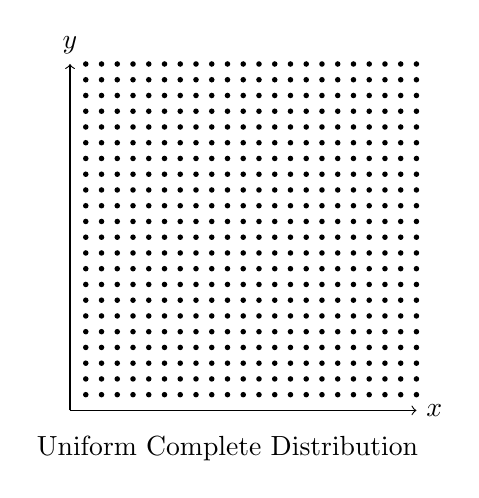
\begin{tikzpicture}[scale=2]
					\foreach \x in {0.1,0.2,...,2.2} {
							\foreach \y in {0.1,0.2,...,2.2} {
									\fill (\x,\y) circle (0.5pt);
								}
						}
					\draw[->] (0,0) -- (2.2,0) node[right] {$x$};
					\draw[->] (0,0) -- (0,2.2) node[above] {$y$};
					\node[below] at (1,-0.1) {Uniform Complete Distribution};
				\end{tikzpicture}
			\end{center}
		\end{column}
		\begin{column}{0.5\textwidth}
			\imagewithcaption{elliptic_curve_integers.png}{Elliptic curve over the integers. Source: Serious Cryptography}
		\end{column}
	\end{columns}
\end{frame}

\begin{frame}{What goes wrong without proper key derivation?}
	\begin{columns}[c]
		\begin{column}{0.5\textwidth}
			\textbf{Example: Curve25519 point as AES key}
			\begin{itemize}
				\item Curve25519 produces 32-byte x-coordinates
				\item But only $\approx 2^{252}$ valid points
				\item AES-256 expects uniform 256-bit keys
			\end{itemize}
			\textbf{Concrete attack scenario:}
			\begin{itemize}
				\item Attacker knows top bits are biased
				\item Can distinguish real keys from random
				\item Reduces effective key space
				\item Makes brute force easier
			\end{itemize}
		\end{column}
		\begin{column}{0.5\textwidth}
			\textbf{Distribution problems:}
			\begin{itemize}
				\item \textbf{Bit bias}: Top 3 bits of x-coordinate never all 1
				\item \textbf{Modular reduction}: $x < 2^{255} - 19$
				\item \textbf{Invalid points}: Half of x-values have no corresponding y
			\end{itemize}
			\begin{alertblock}{Real vulnerability}
				In some protocols, attacker can force specific shared secrets by choosing malicious public keys from small subgroups
			\end{alertblock}
		\end{column}
	\end{columns}
\end{frame}

\begin{frame}{OTR's hand-rolled KDF}
	\begin{itemize}
		\item \textbf{OTR needed multiple keys from one shared secret}
		      \begin{itemize}
			      \item Encryption keys, MAC keys, counter values\ldots
			      \item Needed consistent, deterministic derivation
		      \end{itemize}
		\item \textbf{Their solution (simplified):}
		      \begin{itemize}
			      \item $h_0 = \func{sha256}{s \mathbin{\|} \texttt{0x00}}$
			      \item $h_1 = \func{sha256}{s \mathbin{\|} \texttt{0x01}}$
			      \item $h_2 = \func{sha256}{s \mathbin{\|} \texttt{0x02}}$
			      \item Extract different keys from different hash outputs
		      \end{itemize}
		\item \textbf{Problems with this approach:}
		      \begin{itemize}
			      \item No formal security analysis
			      \item Related-key concerns
			      \item Every protocol invented its own variant
			      \item No standard way to include context/domain separation
		      \end{itemize}
	\end{itemize}
\end{frame}

\begin{frame}{Enter HKDF: HMAC-based Key Derivation Function}
	\begin{columns}[c]
		\begin{column}{0.5\textwidth}
			\textbf{Motivated by real needs:}\footnote{\url{https://appliedcryptography.page/paper/\#hkdf-scheme}}
			\begin{itemize}
				\item OTR, TLS, IPsec all needed KDFs
				\item Each had ad-hoc solutions
				\item Krawczyk (2010) formalized the problem
			\end{itemize}
			\textbf{HKDF Design:}
			\begin{itemize}
				\item \textbf{Extract}: Concentrate entropy
				      \begin{itemize}
					      \item $\texttt{prk} = \func{hmac}{\texttt{salt}, \texttt{ikm}}$
				      \end{itemize}
				\item \textbf{Expand}: Generate keys
				      \begin{itemize}
					      \item $\texttt{okm} = \func{hkdf\text{-}expand}{\texttt{prk}, \texttt{info}, \texttt{len}}$
				      \end{itemize}
			\end{itemize}
		\end{column}
		\begin{column}{0.5\textwidth}
			\textbf{Why HKDF is great:}
			\begin{itemize}
				\item \textbf{Provably secure}
				      \begin{itemize}
					      \item Based on HMAC security
					      \item Extract-then-expand paradigm
				      \end{itemize}
				\item \textbf{Domain separation}
				      \begin{itemize}
					      \item ``info'' parameter for context
					      \item Different contexts $\rightarrow$ different keys
				      \end{itemize}
				\item \textbf{Flexible output}
				      \begin{itemize}
					      \item Generate any length needed
					      \item Multiple keys from one PRK
				      \end{itemize}
				\item \textbf{Now standard}: RFC 5869
			\end{itemize}
		\end{column}
	\end{columns}
\end{frame}

\begin{frame}{HKDF in practice: OTR key derivation}{OTR does not do this, this is an example}
	\begin{columns}[c]
		\begin{column}{0.5\textwidth}
			\textbf{From one secret to many keys:}
			\begin{itemize}
				\item Start with: $s = g^{xy}$
				\item Derive some unique session ID as the salt
				\item \texttt{HKDF(ikm, info, salt, len)}
			\end{itemize}
			\begin{exampleblock}{OTR Key Derivation}
				\ttfamily\scriptsize
				c = HKDF(s, "OTR-ENC-Alice", sessionID, 32)\\
				c' = HKDF(s, "OTR-ENC-Bob", sessionID, 32)\\
				m1 = HKDF(s, "OTR-MAC1-Alice", sessionID, 2)\\
				m1' = HKDF(s, "OTR-MAC1-Bob", sessionID, 32)\\
				m2 = HKDF(s, "OTR-MAC2-Alice", sessionID, 32)\\
				m2' = HKDF(s, "OTR-MAC2-Bob", sessionID, 32)
			\end{exampleblock}
		\end{column}
		\begin{column}{0.5\textwidth}
			\textbf{Domain separation benefits:}
			\begin{itemize}
				\item \textbf{Clear purpose}: Each key has explicit context
				\item \textbf{No key reuse}: Different contexts = different keys
				\item \textbf{Direction-specific}: Alice/Bob get different keys
			\end{itemize}
			\textbf{Compare to ad-hoc approach:}
			\begin{itemize}
				\item No semantic meaning
				\item Easy to mess up counters
				\item No formal analysis
			\end{itemize}
		\end{column}
	\end{columns}
\end{frame}

\section{Back to OTR: Sending and Receiving Messages}

\begin{frame}{OTR: message exchange and ratcheting}
	\begin{itemize}
		\item \textbf{Each message includes:}
		      \begin{itemize}
			      \item The encrypted message itself
			      \item A new ephemeral DH public key share
			      \item MAC authenticating the entire message
		      \end{itemize}
		\item \textbf{On sending/receiving a message:}
		      \begin{enumerate}
			      \item Generate new ephemeral key pair: $x_{\text{new}} \twoheadleftarrow \bits^{\lambda}$
			      \item Include $g^{x_{\text{new}}}$ with the message
			      \item Compute new shared secret: $s_{\text{new}} = g^{x_{\text{new}} \cdot y_{\text{current}}}$
			      \item Derive new keys from $s_{\text{new}}$
			      \item Delete old ephemeral private key
		      \end{enumerate}
		\item \textbf{MAC key revelation (for deniability):}
		      \begin{itemize}
			      \item Once both parties have acknowledged receipt
			      \item Publish the old MAC keys in cleartext
			      \item Anyone could now forge past messages!
			      \item No cryptographic proof of who sent what
		      \end{itemize}
	\end{itemize}
\end{frame}

\begin{frame}{Forward secrecy example: stolen laptop}
	\begin{columns}[c]
		\begin{column}{0.5\textwidth}
			\textbf{The Scenario:}
			\begin{itemize}
				\item You're having an OTR conversation
				\item 30 messages already exchanged
				\item Your laptop gets stolen!
				\item Attacker has:
				      \begin{itemize}
					      \item Your current ephemeral key
					      \item Your long-term identity key
					      \item The OTR client state
				      \end{itemize}
			\end{itemize}
		\end{column}
		\begin{column}{0.5\textwidth}
			\textbf{What the attacker CAN do:}
			\begin{itemize}
				\item Continue the conversation as you
				\item Read messages buffered in memory
				\item Decrypt future messages (until detected)
			\end{itemize}
			\textbf{What the attacker CANNOT do:}
			\begin{itemize}
				\item Decrypt your past 30 messages
				\item Recover deleted ephemeral keys
				\item Prove you sent past messages
			\end{itemize}
		\end{column}
	\end{columns}
\end{frame}

\begin{frame}{Limitations to forward secrecy in practice}
	\begin{columns}[c]
		\begin{column}{0.5\textwidth}
			\textbf{Key erasure challenges:}
			\begin{itemize}
				\item \textbf{Memory persistence}
				      \begin{itemize}
					      \item Keys may remain in RAM
					      \item Swap files on disk
					      \item Hibernation files
					      \item Core dumps
				      \end{itemize}
				\item \textbf{Language/OS limitations}
				      \begin{itemize}
					      \item No guaranteed secure erasure
					      \item Garbage collection delays
					      \item Memory optimization copies
				      \end{itemize}
			\end{itemize}
		\end{column}
		\begin{column}{0.5\textwidth}
			\textbf{Synchronization vs Security:}
			\begin{itemize}
				\item \textbf{The dilemma:}
				      \begin{itemize}
					      \item Messages arrive out of order
					      \item Network delays/retries
					      \item Must decrypt when received
				      \end{itemize}
				\item \textbf{Signal/WhatsApp solution:}
				      \begin{itemize}
					      \item Keep window of old keys
					      \item ``Message key cache''
					      \item Trade-off: usability vs security
				      \end{itemize}
				\item \textbf{Real impact:}
				      \begin{itemize}
					      \item Forward secrecy weakened
					      \item Attack window extended
					      \item But better UX
				      \end{itemize}
			\end{itemize}
		\end{column}
	\end{columns}
\end{frame}

\begin{frame}{Deniability as a security property}
	\begin{columns}[c]
		\begin{column}{0.5\textwidth}
			\textbf{What is deniability?}
			\begin{itemize}
				\item Messages authenticated to recipient
				\item But no cryptographic proof for third parties
				\item \textbf{After conversation:} anyone could have created the transcript
			\end{itemize}
			\textbf{OTR's approach:}
			\begin{itemize}
				\item \textbf{MACs instead of signatures}
				      \begin{itemize}
					      \item Both parties have MAC key
					      \item Either could forge messages
					      \item Old MAC keys revealed
					      \item Now anyone can now forge past messages
				      \end{itemize}
			\end{itemize}
		\end{column}
		\begin{column}{0.5\textwidth}
			\textbf{Contrast with digital signatures:}
			\begin{itemize}
				\item \textbf{PGP-signed email:}
				      \begin{itemize}
					      \item Permanent proof of authorship
					      \item Third party can verify later
					      \item Non-repudiation by design
				      \end{itemize}
				\item \textbf{OTR philosophy:}
				      \begin{itemize}
					      \item Like face-to-face conversation
					      \item No permanent cryptographic record
					      \item Protects against coercion
				      \end{itemize}
			\end{itemize}
		\end{column}
	\end{columns}
\end{frame}

\begin{frame}{The deniability debate: Manning/Lamo case}
	\textbf{The 2010 incident:}
	\begin{itemize}
		\item Chelsea Manning allegedly used OTR with Adrian Lamo
		\item Allegedly discussed classified document leaks
		\item Lamo saved chat logs, gave to FBI
		\item \textbf{Used as evidence in court}
	\end{itemize}
	\textbf{Why deniability failed:}
	\begin{itemize}
		\item Courts don't require cryptographic proof
		\item Context and corroboration matter more
		\item One party (Lamo) testified to authenticity
		\item Technical deniability $\neq$ legal deniability
	\end{itemize}
\end{frame}

\begin{frame}{The deniability debate: Is deniability worth anything?}
	\textbf{Is deniability worth anything?}
	\begin{itemize}
		\item \textbf{Arguments for:}
		      \begin{itemize}
			      \item Prevents automatic mass verification
			      \item Raises doubt about leaked transcripts
			      \item Protects against future proof requirements
		      \end{itemize}
		\item \textbf{Arguments against:}
		      \begin{itemize}
			      \item Courts accept weaker evidence
			      \item Screenshots can be just as damning
			      \item Adds protocol complexity
			      \item Users don't understand it
		      \end{itemize}
	\end{itemize}
	\begin{alertblock}{Open question}
		Does cryptographic deniability provide meaningful real-world protection?
	\end{alertblock}
\end{frame}

\begin{frame}{Attacks on OTR version 2}
	\begin{columns}
		\begin{column}{0.5\textwidth}
			\textbf{Version Rollback Attack}\footnote{\url{https://appliedcryptography.page/paper/\#otr-analysis}}
			\begin{itemize}
				\item Version negotiation happens before authentication
				\item Attacker can force use of older, weaker version
				\item \textbf{Attack scenario:}
				      \begin{itemize}
					      \item Attacker modifies messages to claim only OTRv1
				      \end{itemize}
				\item \textbf{The fix:}
				      \begin{itemize}
					      \item Include version number in AKE
					      \item Authenticate the negotiated version
				      \end{itemize}
			\end{itemize}
		\end{column}
		\begin{column}{0.5\textwidth}
			\textbf{Authentication Failure}
			\begin{itemize}
				\item Mallory can convince Alice she completed AKE with Bob
				\item Bob has no knowledge of this exchange
				\item Only affects AKE completion belief
				\item \textbf{Important limitations:}
				      \begin{itemize}
					      \item No actual MITM possible
					      \item Cannot decrypt messages
					      \item Cannot impersonate either party
				      \end{itemize}
				\item \textbf{Real impact:}
				      \begin{itemize}
					      \item Alice thinks she's secure with Bob
					      \item Sends encrypted messages Bob can't read
				      \end{itemize}
			\end{itemize}
		\end{column}
	\end{columns}
\end{frame}

\begin{frame}{OTRv2 message integrity attack}
	\begin{columns}[c]
		\begin{column}{0.5\textwidth}
			\textbf{Attack Setup:}
			\begin{itemize}
				\item Exploits MAC key revelation + message ordering
				\item Requires network control (active attacker)
			\end{itemize}
			\textbf{Key Insight:}
			\begin{itemize}
				\item Alice reveals MAC keys after ``finishing'' with them
				\item Assumes messages arrive in order, but attacker can delay/reorder messages!
				\item Combined with malleable encryption = attack
			\end{itemize}
		\end{column}
		\begin{column}{0.5\textwidth}
			\textbf{Attack Prerequisites:}
			\begin{itemize}
				\item \textbf{MAC key revelation} for deniability
				\item \textbf{Malleable encryption} (stream cipher)
				\item \textbf{Network control} by attacker
				\item \textbf{Message ordering assumptions}
			\end{itemize}
		\end{column}
	\end{columns}
\end{frame}

\begin{frame}{Message integrity attack: why it works}
	\begin{columns}
		\begin{column}{0.5\textwidth}
			\textbf{Step-by-step:}
			\begin{enumerate}
				\item Alice sends $m_0$ with keys $(x_0, y_0)$
				\item Bob responds with $m_1$ using $(x_1, y_0)$
				\item Alice sees Bob moved to $x_1$, assumes $(x_0, y_0)$ done
				\item Alice publishes MAC keys for $(x_0, y_0)$
				\item Mallory blocks Alice's next message
				\item Mallory creates forged $m'_0$ using:
				      \begin{itemize}
					      \item Published MAC keys
					      \item Malleable encryption
				      \end{itemize}
				\item Bob accepts as delayed message
			\end{enumerate}
		\end{column}
		\begin{column}{0.5\textwidth}
			\textbf{Why Bob accepts it:}
			\begin{itemize}
				\item Message appears to precede $m_1$
				\item Valid MAC (Mallory has the key!)
				\item Network delays are common
				\item No way to detect forgery
			\end{itemize}
			\textbf{Attack Impact:}
			\begin{itemize}
				\item Insert forged messages
				\item Modify past messages
				\item Break conversation integrity
				\item Deniability feature enables attack!
			\end{itemize}
		\end{column}
	\end{columns}
\end{frame}

\begin{frame}{Fixing the message integrity attack}
	\begin{columns}
		\begin{column}{0.5\textwidth}
			\textbf{Potential solutions:}
			\begin{itemize}
				\item \textbf{Delayed MAC revelation}
				      \begin{itemize}
					      \item Wait longer before publishing
					      \item Ensure truly done with keys
				      \end{itemize}
				\item \textbf{Better state machine}
				      \begin{itemize}
					      \item Track message expectations
					      \item Reject out-of-order messages
				      \end{itemize}
			\end{itemize}
		\end{column}
		\begin{column}{0.5\textwidth}
			\textbf{Additional improvements:}
			\begin{itemize}
				\item \textbf{Use authenticated encryption}
				      \begin{itemize}
					      \item Not just MAC + malleable cipher
					      \item Modern AEAD constructions
				      \end{itemize}
				\item \textbf{Include counters in MAC}
				      \begin{itemize}
					      \item Prevent message reordering
					      \item Detect replay attempts
				      \end{itemize}
			\end{itemize}
		\end{column}
	\end{columns}
\end{frame}

\section{Signal}

\begin{frame}{From synchronous to asynchronous messaging}
	\begin{columns}
		\begin{column}{0.5\textwidth}
			\textbf{OTR: Synchronous Protocol}
			\begin{itemize}
				\item Both parties must be online
				\item Real-time key exchange required
				\item Can't send to offline users
				\item \textbf{User experience:}
				      \begin{itemize}
					      \item ``Bob is offline''
					      \item Wait for Bob to come online
					      \item Then initiate secure chat
				      \end{itemize}
				\item Works for MSN Messenger and the early 2000s
				\item Not suitable for mobile era
			\end{itemize}
		\end{column}
		\begin{column}{0.5\textwidth}
			\textbf{Signal: Asynchronous Protocol}
			\begin{itemize}
				\item Send messages anytime
				\item Recipient can be offline
				\item \textbf{SMS-like experience:}
				      \begin{itemize}
					      \item Send message to Bob's phone
					      \item Bob's phone is off
					      \item Bob receives when phone turns on
				      \end{itemize}
				\item \textbf{Challenge:} How to do AKE without Bob?
				\item \textbf{Solution:} Pre-keys on server
			\end{itemize}
		\end{column}
	\end{columns}
\end{frame}

\begin{frame}{OTR version 2: Authenticated Key Exchange}
	\begin{columns}[c]
		\begin{column}{0.5\textwidth}
			\begin{flushleft}
				\begin{tikzpicture}[>=Stealth, scale=0.67, transform shape]
					\node (Alice) at (0,0) {\text{Alice}};
					\node (Bob) at (10,0) {\text{Bob}};
					\draw[->] (0.5,-1) -- (9.5,-1) node[midway,above] {$\begin{array}{rcl}
								r \twoheadleftarrow \bits^{\lambda} \\
								x \twoheadleftarrow \bits^{\lambda} \\
								\func{enc}{r, g^x}, \func{hash}{g^x}
							\end{array}$};
					\draw[<-] (0.5,-2.5) -- (9.5,-2.5) node[midway,above] {$\begin{array}{rcl}
								y \twoheadleftarrow \bits^{\lambda} \\
								g^y
							\end{array}$};
					\draw[->] (0.5,-5.5) -- (9.5,-5.5) node[midway,above] {$\begin{array}{rcl}
								s                                     & =                 & g^{xy}                              \\
								(c, c', m_{1}, m_{1}', m_{2}, m_{2}') & \twoheadleftarrow & \func{hash}{s}                      \\
								M_A                                   & =                 & \func{hmac}{m_{1}, (g^x, g^y, g^A)} \\
								X_A                                   & =                 & (g^A, \func{sign}{A, M_A})          \\
								\multicolumn{3}{c}{r, \func{enc}{c, X_A}, \func{hmac}{m_{2}, \func{enc}{c, X_A}}}
							\end{array}$};
				\end{tikzpicture}
			\end{flushleft}
		\end{column}
		\begin{column}{0.5\textwidth}
			\begin{flushright}
				\begin{tikzpicture}[>=Stealth, scale=0.67, transform shape]
					\draw[<-] (0.5,-1) -- (9.5,-1) node[midway,above] {$\begin{array}{rcl}
								g^x                                    & =                 & \func{dec}{r, \func{enc}{r, g^x}}      \\
								g^x                                    & \overset{?}{=}    & \func{hash}{g^x}                       \\
								s                                      & =                 & g^{xy}                                 \\
								(c, c', m_{1}, m_{1}', m_{2}, m_{2}')  & \twoheadleftarrow & \func{hash}{s}                         \\
								\func{hmac}{m_{2}, \func{enc}{c, X_A}} & \overset{?}{=}    & \func{hmac}{m_{2}, \func{enc}{c, X_A}} \\
								(g^A, \func{sign}{A, M_A})             & =                 & \func{dec}{c, X_A}                     \\
								M_A                                    & =                 & \func{hmac}{m_{1}, (g^x, g^y, g^A)}    \\
								\func{signverif}{g^A, M_A}             & \overset{?}{=}    & \texttt{true}                          \\
								M_B                                    & =                 & \func{hmac}{m_{1}', (g^y, g^x, g^B)}   \\
								X_B                                    & =                 & (g^B, \func{sign}{B, M_B})             \\
								\multicolumn{3}{c}{\func{enc}{c', X_B}, \func{hmac}{m_{2}', \func{enc}{c', X_B}}}
							\end{array}$};
					\draw[->] (0.5,-4) -- (9.5,-4) node[midway,above] {$\begin{array}{rcl}
								\func{hmac}{m_{2}', \func{enc}{c', X_B}} & \overset{?}{=} & \func{hmac}{m_{2}', \func{enc}{c', X_B}} \\
								(g^B, \func{sign}{B, M_B})               & =              & \func{dec}{c', X_B}                      \\
								M_B                                      & =              & \func{hmac}{m_{1}', (g^y, g^x, g^B)}     \\
								\func{signverif}{g^B, M_B}               & \overset{?}{=} & \texttt{true}                            \\
							\end{array}$};
				\end{tikzpicture}
			\end{flushright}
		\end{column}
	\end{columns}
\end{frame}

\begin{frame}{X3DH: Signal's Asynchronous Key Exchange}
	\begin{columns}[c]
		\begin{column}{1\textwidth}
			\vspace{-0.75cm}
			\begin{center}
				\begin{tikzpicture}[>=Stealth, scale=1, transform shape]
					\node (Alice) at (0,0) {\textbf{Alice}};
					\node (Server) at (4,0) {\textbf{Server}};
					\node (Bob) at (8,0) {\textbf{Bob}};
					\draw[<-, thick] (4.5,-0.5) -- (7.5,-0.5) node[midway,above] {\small Upload};
					\node[right, align=left] at (8,-1.5) {$g^B, g^{B}_{spk},$\\[0.25em]$\func{sign}{B, g^{B}_{spk}},$\\[0.25em]$g^{B}_{opk_0} \ldots g^{B}_{opk_{100}}$};
					\draw[->, thick] (0.5,-1) -- (3.5,-1) node[midway,above] {\small Fetch Bob};
					\draw[<-, thick] (0.5,-1.5) -- (3.5,-1.5) node[midway,above] {\small Bundle};
					\node[left, align=right] at (0,-1.5) {$g^B, g^{B}_{spk},$\\[0.25em]$\func{sign}{B, g^{B}_{spk}},$\\[0.25em]$g^{B}_{opk_i}$};
					\node[draw, rounded corners] at (4.25,-4) {$\renewcommand{\arraystretch}{1.5}\begin{array}{rcl}
								\Delta_1 & = & \func{dh}{A, g^{B}_{spk}}                           \\
								\Delta_2 & = & \func{dh}{{A}_{eph_0}, g^B}                         \\
								\Delta_3 & = & \func{dh}{{A}_{eph_0}, g^{B}_{spk}}                 \\
								\Delta_4 & = & \func{dh}{{A}_{eph_0}, g^{B}_{opk_i}}               \\
								S        & = & c_0 \| \Delta_1 \| \Delta_2 \| \Delta_3 \| \Delta_4
							\end{array}$
					};
				\end{tikzpicture}
			\end{center}
		\end{column}
	\end{columns}
\end{frame}

\begin{frame}{X3DH: Signal's Asynchronous Key Exchange}
	\begin{itemize}
		\item $spk$: ``Signed pre-key'': a signed ephemeral key
		      \begin{itemize}
			      \item Replaced every 2 days
		      \end{itemize}
		\item $opk$: ``One-time'' ephemeral pre-key
		      \begin{itemize}
			      \item Bob uploads 100 of them, used only once
		      \end{itemize}
		\item $eph$: Ephemeral keys, generated during the session
		\item $c_0 \ldots c_n$: Various constants found in the protocol
		\item Alice can obtain $S$ even if Bob is offline!
		\item Now, using $S$, Alice can derive a bunch of keys to get the session going
	\end{itemize}
\end{frame}

\begin{frame}{Signal Double Ratchet}
	\vspace{-1.25cm}
	\begin{center}\resizebox{0.7\textwidth}{!}{
			\begin{msc}{}
				\setmscvalues{small}
				\drawframe{none}
				\setlength{\instdist}{7cm}
				\declinst{alice}{}{Alice}
				\declinst{bob}{}{Bob}
				\action*{$\begin{array}{rcl}
							(rk_0, ck_0) & \twoheadleftarrow & \func{hkdf}{S, c_1, c_2}                                                                              \\
							A_{eph_1}    & \twoheadleftarrow & \bits^\lambda                                                                                         \\
							(rk_1, ck_1) & \twoheadleftarrow & \func{hkdf}{\func{dh}{A_{eph_1}, g^{B}_{spk}}, rk_0, c_2}                                             \\
							e_0          & \twoheadleftarrow & \func{hkdf}{\func{hmac}{ck_1, c_3}, c_1, c_4}                                                         \\
							m_0          & =                 & \func{aead-enc}{e_0, \texttt{msg}_0, (g^{A} \| g^{A}_{spk} \| g^{B} \| g^{B}_{spk} \| g^{A}_{eph_1})}
						\end{array}$}{alice}
				\nextlevel[9]
				\mess{$g^{A}, g^{A}_{spk}, g^{A}_{eph_0}, g^{A}_{eph_1}, m_0$}{alice}{bob}
				\nextlevel[1]
				\action*{$\begin{array}{rcl}
							S              & =                 & c_0 \| \func{dh}{B_{spk}, g^{A}} \| \func{dh}{B, g^{A}_{eph_0}} \| \func{dh}{B_{spk}, g^{A}_{eph_0}} \| \func{dh}{{B}_{opk_i}, g^{A}_{eph_0}} \\
							(rk_0, ck_0)   & \twoheadleftarrow & \func{hkdf}{S, c_1, c_2}                                                                                                                      \\
							(rk_1, ck_1)   & \twoheadleftarrow & \func{hkdf}{\func{dh}{B_{spk}, g^{A}_{eph_1}}, rk_0, c_2}                                                                                     \\
							e_0            & \twoheadleftarrow & \func{hkdf}{\func{hmac}{ck_1, c_3}, c_1, c_4}                                                                                                 \\
							\texttt{msg}_0 & =                 & \func{aead-dec}{e_0, m_0, (g^{A} \| g^{A}_{spk} \| g^{B} \| g^{B}_{spk} \| g^{A}_{eph_1})}                                                    \\
							B_{eph_0}      & \twoheadleftarrow & \bits^\lambda                                                                                                                                 \\
							(rk_2, ck_2)   & \twoheadleftarrow & \func{hkdf}{\func{dh}{B_{eph_0}, g^{A}_{eph_1}}, rk_1, c_2}                                                                                   \\
							e_1            & \twoheadleftarrow & \func{hkdf}{\func{hmac}{ck_2, c_3}, c_1, c_4}                                                                                                 \\
							m_1            & =                 & \func{aead-enc}{e_1, \texttt{msg}_1, (g^{B} \| g^{B}_{spk} \| g^{A} \| g^{A}_{spk} \| g^{B}_{eph_0})}
						\end{array}$}{bob}
				\nextlevel[14]
				\mess{$g^{B}_{eph_0}, m_1$}{bob}{alice}
				\nextlevel[1]
				\action*{$\begin{array}{rcl}
							(rk_2, ck_2)   & \twoheadleftarrow & \func{hkdf}{\func{dh}{A_{eph_1}, g^{B}_{eph_0}}, rk_1, c_2}                                \\
							e_1            & \twoheadleftarrow & \func{hkdf}{\func{hmac}{ck_2, c_3}, c_1, c_4}                                              \\
							\texttt{msg}_1 & =                 & \func{aead-dec}{e_1, m_1, (g^{B} \| g^{B}_{spk} \| g^{A} \| g^{A}_{spk} \| g^{B}_{eph_0})}
						\end{array}$}{alice}
				\nextlevel[5]
			\end{msc}
		}\end{center}
\end{frame}

\begin{frame}{Why the Double Ratchet is nice}
	\begin{itemize}
		\item \textbf{Every message gets fresh keys}
		      \begin{itemize}
			      \item Chain key advances: $ck_{i+1} = \func{hmac}{ck_i, c_3}$
			      \item Message key derived: $e_i = \func{hkdf}{\func{hmac}{ck_i, c_3}, c_1, c_4}$
			      \item Old chain keys immediately deleted
			      \item Compromise of $e_i$ reveals nothing about $e_{i-1}$ or $e_{i+1}$
		      \end{itemize}
		\item \textbf{Two types of ratcheting}
		      \begin{itemize}
			      \item \textbf{Symmetric ratchet}: HMAC chain for immediate messages
			      \item \textbf{DH ratchet}: New ephemeral keys when direction changes
			      \item Root key combines both: $(rk_{new}, ck_{new}) = \func{hkdf}{\func{dh}{\text{new ephemerals}}, rk_{old}, c_2}$
		      \end{itemize}
		\item \textbf{Post-compromise security!}
		      \begin{itemize}
			      \item If attacker steals your state at time $t$\ldots
			      \item After one DH ratchet step, they're locked out again
			      \item Fresh randomness from new ephemeral keys
			      \item OTR couldn't do this - required interactive AKE
		      \end{itemize}
	\end{itemize}
\end{frame}

\begin{frame}{Forward Secrecy vs Post-Compromise Security}
	\begin{columns}
		\begin{column}{0.5\textwidth}
			\textbf{Forward Secrecy}
			\begin{itemize}
				\item \textbf{Past messages stay secret}
				\item If keys compromised today, yesterday's messages remain encrypted
				\item ``Looking backward'' protection
				\item \textbf{How it works:}
				      \begin{itemize}
					      \item Delete old keys after use
					      \item Can't decrypt without keys
					      \item Time travel won't help attacker
				      \end{itemize}
				\item \textbf{Example:} Laptop stolen after conversation - past messages safe
			\end{itemize}
		\end{column}
		\begin{column}{0.5\textwidth}
			\textbf{Post-Compromise Security}
			\begin{itemize}
				\item \textbf{Future messages become secret again}
				\item If keys compromised today, tomorrow's messages will be secure
				\item ``Healing'' or ``self-healing'' property
				\item \textbf{How it works:}
				      \begin{itemize}
					      \item Inject fresh randomness
					      \item New ephemeral keys
					      \item Attacker locked out again
				      \end{itemize}
				\item \textbf{Example:} Laptop stolen but recovered - future messages re-secure
			\end{itemize}
		\end{column}
	\end{columns}
\end{frame}

\begin{frame}{Signal's Sealed Sender: the metadata problem}
	\begin{columns}
		\begin{column}{0.5\textwidth}
			\textbf{What E2E encryption doesn't hide:}
			\begin{itemize}
				\item Message contents are protected
				\item But service still sees who talks to whom
				\item Traditional messaging shows:
				      \begin{itemize}
					      \item Sender identity (authentication)
					      \item Recipient identity (routing)
				      \end{itemize}
			\end{itemize}
		\end{column}
		\begin{column}{0.5\textwidth}
			\textbf{Why authentication was needed:}
			\begin{itemize}
				\item Prevent spoofing
				\item Enable rate limiting
				\item Block abuse
				\item Trace bad actors
			\end{itemize}
			\textbf{The challenge:}
			\begin{itemize}
				\item How to hide sender from service
				\item While preventing abuse?
			\end{itemize}
		\end{column}
	\end{columns}
\end{frame}

\begin{frame}{Signal's Sealed Sender: the solution}
	\begin{columns}
		\begin{column}{0.5\textwidth}
			\textbf{Sender Certificates}
			\begin{itemize}
				\item Short-lived, signed by service
				\item Contains:
				      \begin{itemize}
					      \item Phone number
					      \item Identity key
					      \item Expiry timestamp
				      \end{itemize}
				\item Included inside encrypted envelope from Alice to Bob
				\item Service can see it at issuance, but not while it's inside encrypted envelope.
			\end{itemize}
		\end{column}
		\begin{column}{0.5\textwidth}
			\textbf{Delivery Tokens}
			\begin{itemize}
				\item 96-bit token derived from profile key
				\item Required to send sealed messages
				\item Shared via existing profile system
				\item Acts as anti-abuse mechanism
			\end{itemize}
			\textbf{Trade-off:}
			\begin{itemize}
				\item Default: Only contacts can use sealed sender
				\item Optional: Accept from anyone (more spam risk)
			\end{itemize}
		\end{column}
	\end{columns}
\end{frame}

\begin{frame}{Sealed Sender: technical details}
	\textbf{Double Encryption Approach:}
	\begin{enumerate}
		\item Message encrypted with Signal Protocol as usual
		\item Envelope (sender cert + ciphertext) encrypted to recipient's identity key
		\item Service sees only encrypted blob + delivery token
	\end{enumerate}
	\textbf{Envelope Encryption (simplified):}
	\begin{itemize}
		\item Generate ephemeral key pair: $(e_{pub}, e_{priv})$
		\item ECDH with recipient's identity key
		\item Derive encryption keys via HKDF
		\item Encrypt sender identity + certificate
		\item Second layer using sender's identity key for authentication
	\end{itemize}
	\begin{alertblock}{Result}
		Service can route messages without knowing sender identity
	\end{alertblock}
\end{frame}

\begin{frame}{Sealed Sender: does it really work?}
	\begin{columns}[c]
		\begin{column}{0.6\textwidth}
			\begin{itemize}
				\item \textbf{The Attack (2021): Statistical Disclosure}\footnote{\url{https://appliedcryptography.page/paper/\#sealed-sender}}
				      \begin{itemize}
					      \item Sealed sender hides who sent the message
					      \item But delivery receipts create a timing pattern
					      \item When Bob receives a message, he often replies quickly
					      \item This creates a ``reply epoch'' - a time window
				      \end{itemize}
				\item \textbf{The Clever Observation:}
				      \begin{itemize}
					      \item Alice sends to Bob \rightarrow\ Bob likely replies within epoch
					      \item Other users also send/receive during this time
					      \item But Alice appears more often in Bob's reply epochs
				      \end{itemize}
			\end{itemize}
		\end{column}
		\begin{column}{0.4\textwidth}
			\begin{itemize}
				\item \textbf{The Attack Algorithm:}
				      \begin{enumerate}
					      \item Monitor when Bob receives messages
					      \item Count who receives messages right after (target epochs)
					      \item Compare to random time windows
					      \item Alice's count grows, others stay near zero
					      \item After just a few messages: Bob's contacts revealed!
				      \end{enumerate}
			\end{itemize}
		\end{column}
	\end{columns}
\end{frame}

\begin{frame}{Can your message truly be secure after a hack?}
	\begin{columns}[c]
		\begin{column}{1\textwidth}
			\begin{center}
				\Large \textbf{The Promise and Reality of Post-Compromise Security}\footnote{\url{https://appliedcryptography.page/paper/\#pcs-impossibility}}
			\end{center}
			\vspace{1em}
			\begin{itemize}
				\item Based on: ``Impossibility Results for Post-Compromise Security'' by Cremers, Medinger, and Naska (2024)
				\item \textbf{Spoiler:} The answer might surprise you\ldots
			\end{itemize}
		\end{column}
	\end{columns}
\end{frame}

\begin{frame}{The Dream: Self-Healing Security}
	\begin{columns}[c]
		\begin{column}{0.5\textwidth}
			\textbf{The Promise of PCS:}
			\begin{itemize}
				\item Your phone gets hacked today
				\item Attacker reads all your secrets
				\item But tomorrow\ldots
				\item \textbf{Magic happens!}
				\item Future messages become secure again
				\item Attacker is ``locked out''
			\end{itemize}
		\end{column}
		\begin{column}{0.5\textwidth}
			\textbf{How it ``works'':}
			\begin{itemize}
				\item Continuously inject fresh randomness
				\item Update keys with every message
				\item If attacker misses an update\ldots
				\item They can't decrypt future messages!
				\item Like changing locks after a break-in
			\end{itemize}
		\end{column}
	\end{columns}
	\begin{alertblock}{Question for the class}
		Does this sound too good to be true?
	\end{alertblock}
\end{frame}

\begin{frame}{PCS reality check}
	\begin{columns}[c]
		\begin{column}{0.5\textwidth}
			\textbf{Academic papers say:}
			\begin{itemize}
				\item ``Signal Protocol achieves PCS!''
				\item ``Double Ratchet provides healing!''
				\item ``Proven secure!''
				\item Lots of formal proofs! Wow!
			\end{itemize}
		\end{column}
		\begin{column}{0.5\textwidth}
			\textbf{This paper says:}
			\begin{itemize}
				\item Wait, not so fast\ldots
				\item Those proofs assume perfect conditions
				\item Real apps $\neq$ Academic protocols
				\item \textbf{Users don't actually get PCS!}
			\end{itemize}
		\end{column}
	\end{columns}
\end{frame}

\begin{frame}{Phones live in the real world}
	\textbf{Things that happen to real phones:}
	\begin{itemize}
		\item \textbf{Hardware failures:} Bit flips, memory corruption
		\item \textbf{Software issues:} App crashes, OS updates
		\item \textbf{User actions:} Restore from backup, reinstall apps
		\item \textbf{Physical events:} Drop phone in toilet
	\end{itemize}
	\textbf{What happens to your chats when these occur?}
	\begin{itemize}
		\item Academic answer: ``You're locked out forever!''
		\item Real-world requirement: ``I need to keep chatting!''
		\item If WhatsApp doesn't meet that requirement, it will lose users
	\end{itemize}
\end{frame}

\begin{frame}{Sessions all the way down}
	\begin{columns}[c]
		\begin{column}{0.5\textwidth}
			\textbf{What users see:}
			\begin{itemize}
				\item One conversation with Bob
				\item Linear list of messages
				\item Simple and clean
			\end{itemize}
		\end{column}
		\begin{column}{0.5\textwidth}
			\textbf{What's really happening:}
			\begin{itemize}
				\item Multiple concurrent ``sessions''
				\item Signal allows up to \textbf{40 sessions!}
				      \begin{itemize}
					      \item WhatsApp even more, I believe
				      \end{itemize}
				\item Each can be compromised separately
				\item Attacker can start new ones
			\end{itemize}
		\end{column}
	\end{columns}
	\begin{block}{The Impossibility Result}
		If your app must handle state loss (all real apps do), then full conversation-level PCS is \textbf{mathematically impossible}
	\end{block}
\end{frame}

\begin{frame}{Why 40 sessions?}
	\textbf{Signal's Magic Number: 40}
	\begin{itemize}
		\item Not arbitrary - represents a design choice
		\item Each session = tolerance for one ``desync event''
		\item More sessions = Better usability, Worse security
	\end{itemize}
	\begin{columns}[c]
		\begin{column}{0.5\textwidth}
			\textbf{N = 1 (Ultra secure)}
			\begin{itemize}
				\item Minimal attack surface
				\item Constant ``can't decrypt'' errors
				\item Messages lost during network delays
			\end{itemize}
		\end{column}
		\begin{column}{0.5\textwidth}
			\textbf{N = 40 (Signal's choice)}
			\begin{itemize}
				\item Handles many failure scenarios
				\item Good user experience
				\item 40 ways for attacker to get in!
			\end{itemize}
		\end{column}
	\end{columns}
\end{frame}

\begin{frame}{Using Tamarin to crush dreams}
	\textbf{How they proved the impossibility:}
	\begin{enumerate}
		\item Model abstract communication system in Tamarin prover
		\item Add real-world requirements:
		      \begin{itemize}
			      \item Must handle dynamic state loss (crashes, backups)
			      \item Must handle static state loss (lost devices)
			      \item Must allow recovery to continue chatting
		      \end{itemize}
		\item Try to prove PCS property holds\ldots
		\item \textbf{Tamarin finds counterexamples!}
	\end{enumerate}
\end{frame}

\begin{frame}{So what can we do?}
	\textbf{If we can't have perfect PCS, can we do better?}
	\begin{itemize}
		\item \textbf{Reduce session count:} Maybe N = 2 instead of 40?
		\item \textbf{Sequential sessions:} Old sessions can only receive, not send
		\item \textbf{Time limits:} Delete old sessions after time T
		\item \textbf{UI warnings:} Highlight messages from old sessions
	\end{itemize}
	\textbf{But remember:}
	\begin{itemize}
		\item These are band-aids, not cures
		\item Fundamental trade-off remains
		\item Perfect security = Unusable app
	\end{itemize}
\end{frame}

\begin{frame}{Discussion time}
	\begin{columns}[c]
		\begin{column}{0.7\textwidth}
			\begin{enumerate}
				\item \textbf{Is post-compromise security just security theater?}
				      \begin{itemize}
					      \item If users don't actually get it, why do we pretend?
					      \item Marketing vs. reality?
				      \end{itemize}
				\item \textbf{What would you choose?}
				      \begin{itemize}
					      \item Ultra-secure but breaks constantly?
					      \item Works smoothly but weaker guarantees?
				      \end{itemize}
				\item \textbf{Can we do better?}
				      \begin{itemize}
					      \item Hardware security modules?
					      \item Out-of-band verification?
					      \item Just give up on state loss resilience?
				      \end{itemize}
				\item \textbf{Who's being honest with users?}
				      \begin{itemize}
					      \item Should apps disclose these limitations?
					      \item Do users even care?
				      \end{itemize}
			\end{enumerate}
		\end{column}
		\begin{column}{0.3\textwidth}
			\imagewithcaption{noelle_spamton.png}{Academia versus the real world}
		\end{column}
	\end{columns}
\end{frame}

\section{Telegram}

\begin{frame}{What about Telegram?}
	\begin{columns}
		\begin{column}{0.5\textwidth}
			\textbf{Telegram's Approach}
			\begin{itemize}
				\item Two modes: Cloud chats vs Secret chats
				\item Cloud chats: Encrypted to server, not E2E
				\item Secret chats: Custom MTProto 2.0 protocol
				\item Only available in 1-on-1 conversations
				\item Must be explicitly enabled
			\end{itemize}
		\end{column}
		\begin{column}{0.5\textwidth}
			\textbf{Key Differences from Signal}
			\begin{itemize}
				\item Most users never use secret chats
				\item Custom crypto instead of proven protocols
				\item Server can read most messages
				\item Focus on features over security
				\item Different threat model assumptions
			\end{itemize}
		\end{column}
	\end{columns}
	\begin{alertblock}{Security Reality}
		Despite marketing, most Telegram usage is \textbf{not} end-to-end encrypted
	\end{alertblock}
\end{frame}

\begin{frame}{Telegram's MTProto}
	\textbf{What Telegram Did}
	\begin{itemize}
		\item Designed custom encryption protocol
		\item Ignored existing academic work
		\item No formal security analysis initially
		\item Multiple versions after vulnerabilities found
	\end{itemize}
	\textbf{The Cryptographic Community Response}
	\begin{itemize}
		\item ``Don't roll your own crypto!''
		\item Multiple published attacks
		\item Academic papers showing weaknesses
		\item Telegram's defensive responses
	\end{itemize}
\end{frame}

\begin{frame}{Why Telegram made these choices}
	\begin{itemize}
		\item \textbf{Server-side features require plaintext access:}
		      \begin{itemize}
			      \item Cloud sync across unlimited devices
			      \item Powerful search across all messages
			      \item Large file sharing and streaming
			      \item Bots and integrations
			      \item Message editing and deletion
		      \end{itemize}
		\item \textbf{Different threat model:}
		      \begin{itemize}
			      \item ``We don't trust governments, but we trust ourselves''
			      \item Emphasis on government censorship resistance
			      \item Less focus on protecting from service provider
		      \end{itemize}
		\item \textbf{User experience priorities:}
		      \begin{itemize}
			      \item Instant sync, no waiting for key exchange
			      \item Works the same across all platforms
			      \item No ``this message couldn't be decrypted'' errors
		      \end{itemize}
	\end{itemize}
\end{frame}

\begin{frame}{The Telegram Paradox}
	\begin{columns}[c]
		\begin{column}{0.5\textwidth}
			\textbf{What activists think they're getting:}
			\begin{itemize}
				\item End-to-end encrypted messaging
				\item Protection from government surveillance
				\item Secure communication platform
				\item ``Telegram is encrypted, right?''
			\end{itemize}
		\end{column}
		\begin{column}{0.5\textwidth}
			\textbf{What they're actually getting:}
			\begin{itemize}
				\item Messages readable by Telegram servers
				\item Subject to legal requests and seizure
				\item Only secret chats are E2E encrypted
				\item Most users never enable secret chats
			\end{itemize}
		\end{column}
	\end{columns}
	\begin{alertblock}{Real-world Impact}
		Pavel Durov can read your Telegram chats at his discretion
	\end{alertblock}
\end{frame}

\section{Group Secure Messaging}

\begin{frame}{The Group Messaging Problem}
	\begin{columns}[c]
		\begin{column}{0.5\textwidth}
			\textbf{Two-party protocols work great for\ldots two parties}
			\begin{itemize}
				\item Signal Protocol: Alice $\leftrightarrow$ Bob
				\item OTR: Real-time 1-on-1 chat
				\item X3DH: Asynchronous key agreement
				\item Double Ratchet: Forward secrecy
			\end{itemize}
			\textbf{But what about groups?}
			\begin{itemize}
				\item Family group chat (5 people)
				\item Work team (20 people)
				\item Community groups (100+ people)
			\end{itemize}
		\end{column}
		\begin{column}{0.5\textwidth}
			\textbf{Security challenges:}
			\begin{itemize}
				\item Members join and leave
				\item Forward secrecy for leavers
				\item Post-compromise security
				\item Scalability requirements
			\end{itemize}
		\end{column}
	\end{columns}
\end{frame}

\begin{frame}{How Signal/WhatsApp handle groups today}
	\textbf{The Pairwise Channel Approach}
	\begin{itemize}
		\item No true group protocol
		\item Sender encrypts to each member
		\item For $n$ members: $n-1$ encryptions
		\item Each member has separate ratchet
	\end{itemize}
	\textbf{Problems with this approach:}
	\begin{itemize}
		\item \textbf{Linear scaling:} $O(n)$ work per message
		\item \textbf{Bandwidth:} Upload grows with group size
		\item \textbf{Battery drain:} More crypto operations
		\item \textbf{Consistency:} Members may see different states
	\end{itemize}
\end{frame}

\begin{frame}{WhatsApp's approach: sender keys}
	\begin{columns}[c]
		\begin{column}{0.5\textwidth}
			\textbf{How Sender Keys Work:}
			\begin{itemize}
				\item Each group member has a ``sender key''
				\item Shared with all other members
				\item One encryption per message (not per recipient!)
			\end{itemize}
			\textbf{Sender Key Components:}
			\begin{itemize}
				\item $SK = (spk, ck)$
				\item $spk$: Public signature key
				\item $ck$: Symmetric chain key
				\item Chain key ratchets forward
			\end{itemize}
		\end{column}
		\begin{column}{0.5\textwidth}
			\textbf{Sending a Message:}
			\begin{enumerate}
				\item Derive message key: $mk = H_1(ck)$
				\item Encrypt: $c = \func{enc}{mk, m}$
				\item Sign: $\sigma = \func{sign}{ssk, c}$
				\item Erase $mk$ immediately
				\item Ratchet: $ck_{new} = H_2(ck)$
			\end{enumerate}
			\textbf{Benefits:}
			\begin{itemize}
				\item $O(1)$ encryptions per message
				\item Handles out-of-order delivery
				\item Scales to large groups
			\end{itemize}
		\end{column}
	\end{columns}
\end{frame}

\begin{frame}{WhatsApp's approach: sender keys}
	\bigimagewithcaption{sender_keys.png}{Source: David Balbás, Daniel Collins and Phillip Gajland, \textit{WhatsUpp with Sender Keys? Analysis, Improvements and Security Proofs}, IACR Asiacrypt, 2023.}
\end{frame}

\begin{frame}{Sender keys: trade-offs}
	\begin{columns}[c]
		\begin{column}{0.5\textwidth}
			\textbf{What we gain:}
			\begin{itemize}
				\item \textbf{Efficiency}: Single encryption
				\item \textbf{Scalability}: Works for 256+ members\footnote{Recently increased to 1,024.}
				\item \textbf{Battery life}: Less crypto work
				\item \textbf{Bandwidth}: Constant message size
			\end{itemize}
		\end{column}
		\begin{column}{0.5\textwidth}
			\textbf{What we lose:}
			\begin{itemize}
				\item Weaker forward secrecy
				\item Weaker post-compromise security
				\item Malicious server can add/remove parties
			\end{itemize}
		\end{column}
	\end{columns}
\end{frame}

\begin{frame}{Enter MLS: Messaging Layer Security}
	\begin{columns}[c]
		\begin{column}{0.5\textwidth}
			\textbf{IETF Standard (RFC 9420, July 2023)}
			\begin{itemize}
				\item Designed for efficient group messaging
				\item Single encryption per message
				\item Logarithmic scaling: $O(\log n)$
				\item Native group key agreement
			\end{itemize}
		\end{column}
		\begin{column}{0.5\textwidth}
			\begin{itemize}
				\item \textbf{Group key agreement}: All members share same key
				\item \textbf{Ratcheting epochs}: Keys evolve over time
				\item \textbf{Forward secrecy}: Past epochs stay secure
				\item \textbf{Post-compromise security}: Healing after breach
			\end{itemize}
		\end{column}
	\end{columns}
\end{frame}

\begin{frame}{Quick note: HPKE}
	\begin{columns}[c]
		\begin{column}{0.5\textwidth}
			\textbf{Hybrid Public Key Encryption (RFC 9180)\footnote{\url{https://www.rfc-editor.org/rfc/rfc9180.html}}}
			\begin{itemize}
				\item Combines asymmetric + symmetric crypto
				\item Encrypts to public key, no interaction needed
				\item Used in TLS 1.3, MLS, and more
			\end{itemize}
			\textbf{Two-step process:}
			\begin{enumerate}
				\item \textbf{Encapsulation}: Generate shared secret
				\item \textbf{Seal}: Encrypt data with that secret
			\end{enumerate}
		\end{column}
		\begin{column}{0.5\textwidth}
			\textbf{Simple Example:}
			\begin{exampleblock}{Sender (Alice)}
				\ttfamily\scriptsize
				// Bob's public key: pk\_bob\\
				(enc, ctx) = HPKE.Setup(pk\_bob)\\
				ciphertext = ctx.Seal("Hello Bob!")\\
				// Send: (enc, ciphertext)
			\end{exampleblock}
			\begin{exampleblock}{Receiver (Bob)}
				\ttfamily\scriptsize
				// Bob's private key: sk\_bob\\
				ctx = HPKE.Setup(enc, sk\_bob)\\
				plaintext = ctx.Open(ciphertext)\\
				// plaintext = "Hello Bob!"
			\end{exampleblock}
			\textbf{Key benefit:} One-shot encryption without prior key exchange!
		\end{column}
	\end{columns}
\end{frame}

\begin{frame}{TreeKEM: use a tree to manage group AKE}
	\begin{columns}[c]
		\begin{column}{0.5\textwidth}
			\textbf{Tree of Subgroups:}
			\begin{itemize}
				\item Each node = subgroup with secret (e.g., $s_{abc}$)
				\item Corresponding public key (e.g., $\texttt{pk}_{abc}$)
				\item Example: $s_{abcde}$ is the group key
			\end{itemize}
			\textbf{Member Knowledge:}
			\begin{itemize}
				\item Member $b$ knows: $s_{ab}$, $s_{abc}$, $s_{abcde}$
				\item Only secrets on path to root
				\item Cannot compute sibling secrets
			\end{itemize}
		\end{column}
		\begin{column}{0.5\textwidth}
			\textbf{Updating Keys (Commit):}
			\begin{itemize}
				\item Member $b$ updates its path:
				      \begin{itemize}
					      \item $s_{ab} \rightarrow s'_{ab}$
					      \item $s_{abc} \rightarrow s'_{abc}$
					      \item $s_{abcde} \rightarrow s'_{abcde}$
				      \end{itemize}
				\item Encrypt to siblings:
				      \begin{itemize}
					      \item $\func{hpke}{\texttt{pk}_c, s'_{abc}}$
					      \item $\func{hpke}{\texttt{pk}_{de}, s'_{abcde}}$
				      \end{itemize}
			\end{itemize}
			\begin{alertblock}{Efficiency Win}
				For $n$ members: Only $\log(n)$ encryptions!\\
				Example: 8 members = 3 encryptions
			\end{alertblock}
		\end{column}
	\end{columns}
\end{frame}

\begin{frame}{TreeKEM}
	\bigimagewithcaption{treekem_a.png}{Source: Théophile Wallez}
\end{frame}

\begin{frame}{TreeKEM}
	\bigimagewithcaption{treekem_b.png}{Source: Théophile Wallez}
\end{frame}

\begin{frame}{MLS: reality check}
	\begin{columns}[c]
		\begin{column}{0.5\textwidth}
			\textbf{The Complexity Problem:}
			\begin{itemize}
				\item \textbf{Massive specification}: RFC 9420 is 132 pages!
				\item \textbf{Implementation nightmare}:
				      \begin{itemize}
					      \item Multiple tree operations
					      \item Complex state management
					      \item Intricate error handling
				      \end{itemize}
				\item \textbf{Correctness is hard}:
				      \begin{itemize}
					      \item Easy to get wrong
					      \item Subtle security bugs
					      \item Few complete implementations
				      \end{itemize}
			\end{itemize}
		\end{column}
		\begin{column}{0.5\textwidth}
			\textbf{Developer Hostility:}
			\begin{itemize}
				\item \textbf{No standard API}:
				      \begin{itemize}
					      \item Each implementation different
					      \item No drop-in replacement
					      \item Steep learning curve
				      \end{itemize}
				\item \textbf{Infrastructure requirements}:
				      \begin{itemize}
					      \item Need custom delivery service
					      \item Complex server-side logic
					      \item State synchronization issues
				      \end{itemize}
			\end{itemize}
		\end{column}
	\end{columns}
\end{frame}

\begin{frame}[plain]
	\titlepage
\end{frame}
\end{document}
